\section{Crotch absorber}
\subsection{Raytracing}
For the power density of the input beam the contribution from two SESAME bending magnets (upstream and downstream of the ID) was considered in addition to the BEATS 3PW. The modified magnetic field profile used for the calculation is shown in Figure \ref{fig:modifiedfieldprofile}. \\
\begin{figure}[ht]
\centering
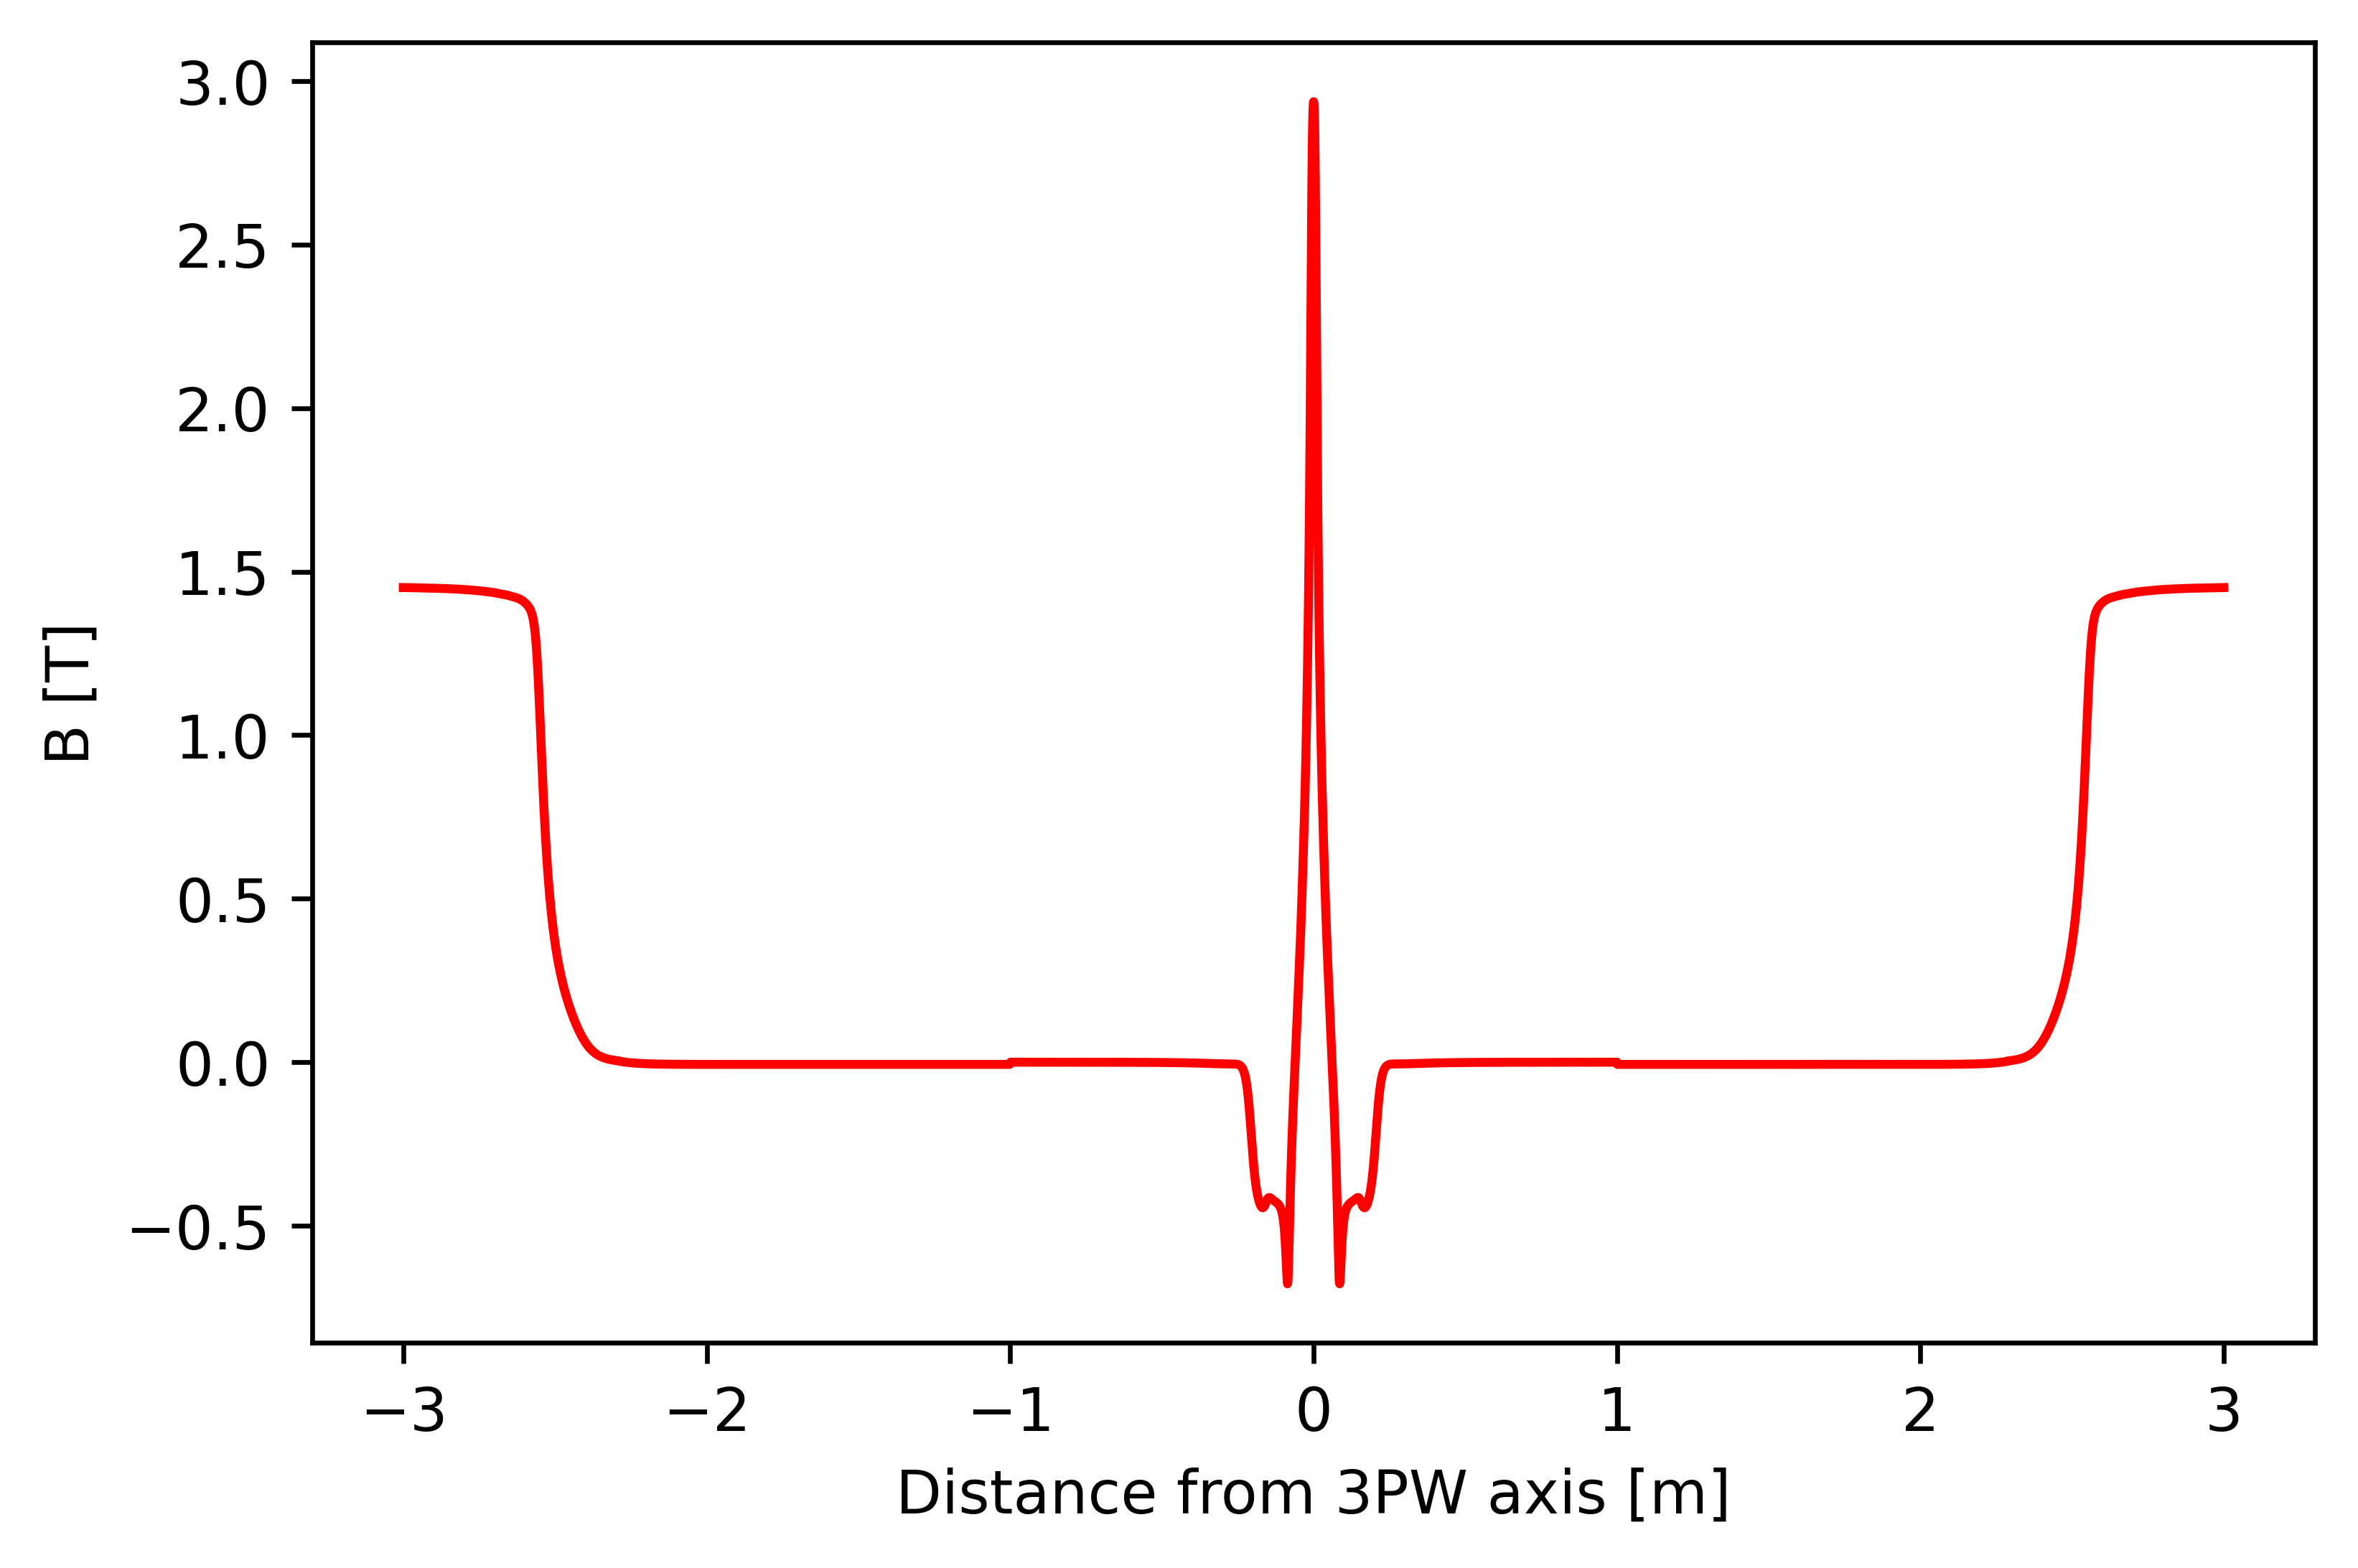
\includegraphics[width=0.8\textwidth]{images/modified_field_profile.png}
\caption{\label{fig:modifiedfieldprofile} Magnetic field profile modified considering the BEATS source plus two BMs (up and downstream) for calculation of the power load on the crotch absorber.}
\end{figure}

\subsection{Design}
The crotch absorber entrance is positioned 4.1 m from the ID photon source. We will modify one of the existing SESAME absorbers and machine an aperture of $12.3mm \times 3.28 mm$, for an acceptance of $3.0 mrad \times 0.8  mrad$. 

\subsection{Input beam}
The power density profile of the beam at the crotch absorber entrance is shown in Figure \ref{fig:power_profile_crotch}. Raw data can be found in the \powerprofilesurl. \\
\begin{figure}[ht]
\centering
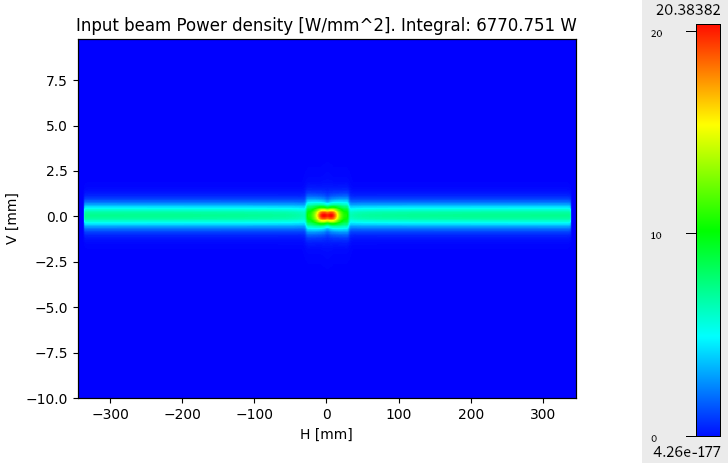
\includegraphics[width=0.8\textwidth]{images/power_profile_crotch.png}
\caption{\label{fig:power_profile_crotch} Power density profile at the crotch absorber entrance (4.1 m from source).}
\end{figure}